\documentclass{article}
\usepackage[utf8]{inputenc}
\usepackage[english]{babel}

\DeclareUnicodeCharacter{2212}{-}

\usepackage{amsfonts}
\usepackage{amsthm}
\usepackage{amssymb}
\usepackage{amsmath}
\usepackage{tikz}
\usetikzlibrary{shapes.arrows,chains,trees}

\theoremstyle{definition}
\newtheorem{definition}{Definition}[section]
\newtheorem{theorem}{Theorem}[section]
\newtheorem{hypothesis}{Hypothesis}[section]
\newtheorem{example}{Example}[section]

\newcommand{\G}{\mathcal{G}}

\setlength{\parindent}{0pt}

\begin{document}

\tableofcontents
\pagebreak

\section{Problems}
Firstly we shall look at two problems which belong to the complexity class NP.

\textbf{Traveling Sales Person}\\
Consider a finite set $N$ of cities; $\{1, 2 \dots n\}$. The distance, or cost,
of traveling between cities $i$ and $j$ is given by $D(i,j)$ where $D$
is a symmetric matrix.

$$\forall\ i, j\quad D(i,J) \in \mathbb{N}\quad D(i,j) = D(j,i)$$

The problem is to find a path, or permutation, of
cities where each city appears exactly once in the path and the total
cost is minimised.

The brute force solution is to consider all paths, doing this would require
considering $!n$ paths.

\textbf{Boolean Formula Satisfiability}\\
A boolean formula consists of the logical binary operators $(\land, \lor, \neg)$
and a finite set of variables $X$ where each variable can be either true or false.
The problem consists of deciding if there exists a set of values for the variables $X$
which results in the boolean formula being true.

$$(x_1 \land x_2) \land \neg x_3$$

$$(x_1 \land x_2) \land \neg x_1$$

A brute force solution would be to consider all $2^{|X|}$ possible assignments.

The link between these two problems is the na\"ive brute force solution is not
tractable for large values of $n$.

\begin{itemize}
    \item \textbf{Input}: Real numbers $x_1,\dots x_n$
    \item \textbf{Output}: Yes iff there exists a subset of $x_i$ which sum to 1.
\end{itemize}

\textit{Traveling Sales Person}\\
\begin{itemize}
    \item \textbf{Inputs}:
    \item \textbf{Output}:
\end{itemize}
Consider a finite set $N$ of cities; $\{1, 2 \dots n\}$. The distance, or cost,
of traveling between cities $i$ and $j$ is given by $D(i,j)$ where $D$
is a symmetric matrix.

$$\forall\ i, j\quad D(i,J) \in \mathbb{N}\quad D(i,j) = D(j,i)$$

The problem is to find a path, or permutation, of
cities where each city appears exactly once in the path and the total
cost is minimised.

The brute force solution is to consider all paths, doing this would require
considering $!n$ paths.

\textit{Traveling Sales Person (Yes-No Version)}\\
\begin{itemize}
    \item \textbf{Inputs}:
    \item \textbf{Output}:
\end{itemize}
Consider a finite set $N$ of cities; $\{1, 2 \dots n\}$. The distance, or cost,
of traveling between cities $i$ and $j$ is given by $D(i,j)$ where $D$
is a symmetric matrix.

$$\forall\ i, j\quad D(i,J) \in \mathbb{N}\quad D(i,j) = D(j,i)$$

The problem is to find a path, or permutation, of
cities where each city appears exactly once in the path and the total
cost is minimised.

\textit{Boolean Formula Satisfiability}\\
\begin{itemize}
    \item \textbf{Inputs}:
    \item \textbf{Output}:
\end{itemize}
A boolean formula consists of the logical binary operators $(\land, \lor, \neg)$
and a finite set of variables $X$ where each variable can be either true or false.
The problem consists of deciding if there exists a set of values for the variables $X$
which results in the boolean formula being true.

$$(x_1 \land x_2) \land \neg x_3$$

$$(x_1 \land x_2) \land \neg x_1$$

A brute force solution would be to consider all $2^{|X|}$ possible assignments.

The link between these two problems is the na\"ive brute force solution is not
tractable for large values of $n$.

\textit{Knapsack Problem}\\
\begin{itemize}
    \item \textbf{Input}: Real numbers $x_1,\dots x_n$
    \item \textbf{Output}: Yes iff there exists a subset of $x_i$ which sum to 1.
\end{itemize}


\pagebreak
\section{Turing Machines}
\subsection{Deterministic Turing Machines}
%TODO
What do Turing machines do? Why are we looking at them?
Conceptually a turing machine is a \textit{tape} which is infinite in both directions,
the input is writen on this tape with the rest of the tape being blank. We have a head
which can read and write to the tape. The machine moves across the tape acording to
a transition function until it reaches a terminal state which produces a yes or no result.

\begin{center}
    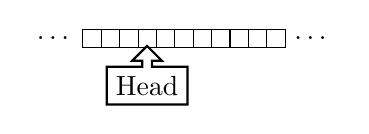
\begin{tikzpicture}[
            start chain=1 going right,start chain=2 going below,node distance=-0.15mm
        ]
        \node [on chain=1] at (-1.5,-.4) {\ldots};
        \foreach \x in {1,2,...,11} {\x, \node [draw,on chain=1] {}; }
        \node [
            name=k,
            arrow box,
            on chain=2,
            arrow box arrows={north:.25cm},
            draw=black,thick
            ] at (-0.335,-1) {Head};
        \node [name=r,on chain=1] {\ldots};
    \end{tikzpicture}
\end{center}

\begin{definition}
    Formally a Turing machine consists of
    \begin{itemize}
        \item A \textit{tape alphabet} $\Gamma$ $\{a_1, a_2 \dots a_n, \beta\}$,
            where $a_i$ is a symbol, and $\beta$ is the blank or empty symbol.
        \item An \textit{input alphabet} $\Sigma$
            where $\Sigma \subset \Gamma \setminus \{\beta\}$.
        \item A set of states $Q$ $\{q_0, q_1 \dots q_m, q_y, q_n\}$ where $q_0$ is the
            initial state, $q_y$ is the terminal yes state, and $q_n$ is the terminal no state.
            $Q\prime = Q \setminus \{q_y,q_n\}$, i.e. the non-terminal states.
        \item A transition function $\delta$,
            where $\delta\ :\ (Q\prime \times \Gamma) \rightarrow
            (Q \times \Sigma \times \{L,S,R\})$.
            What this means is we look at a pair of a non-terminal state
            and a symbol from the alphabet;
            given this we enter a new state $q \in Q$,
            we write to the tape a symbol $a \in \Gamma$,
            and we stay or move the head left or right $(\{L,S,R\})$.
    \end{itemize}
\end{definition}

\begin{definition}
    Given an input $n$ and a Turing machine,
    $T(n)$ is the amount of times the transition function 
    $\delta$ must be applied to reach a terminal state.
\end{definition}

\textbf{Even or odd}
\begin{example}
    In this example we will present a turing machine to decide if a number is even.
    \begin{itemize}
        \item Input: a number $x \in \mathbb{Z}$ in unary form; i.e. $\{1 = X, 2 = XX\dots\}$,
            thus $\Sigma = \{X\}$.
        \item Output: yes iff $x$ is even, otherwise no. I.e. the turing machine will finish
            in state $q_y$ iff $x$ is even.
        \item Transition function $\delta$ is described as a matrix below with the states
            $Q\prime = \{q_0,q_1\}$ and $\Sigma = \{X,\beta\}$,
            output is $(Q \times \Sigma \times \{L,S,R\})$.
            \begin{center}
                \begin{tabular}{ c c c }
                    & $q_0$           & $q_1$           \\
                    X    & ($q_1,\beta,R$) & ($q_0,\beta,R$) \\
                    $\beta$ & ($q_y,\beta,S$) & ($q_n,\beta,S$) \\
                \end{tabular}
            \end{center}
    \end{itemize}
    For this Turing machine $T(n) = n + 1$.
\end{example}

\textbf{Recognising Palindromes}\\
A palindrome is any word such that the reversed word is equal to the word itself,
consider the alphabet $\Gamma = \{a,b\}$, examples of palindromes would be $a, aa, aba$ etc.
Can we construct a Turing machine which recognises palindromes for the alphabet $\Gamma$?

We can, we simply move forward and backward checking each letter at opposite ends is the same,
until the entire word has been checked.
This means for palindromes $T(n)$ is equal to $n + (n - 1) \dots + 1$. Thus
$$T(n) = \frac{n^2 + n}{2}$$

However in non palindrome cases, say $aaa \dots ab$, then $T(n)$ is very small.

\subsection{Non-Deterministic Turing Machines}
\begin{definition}
    \textit{Nondeterministic Turing Machine (NTM)} has
    the same constituent elements as a deterministic Turing Machine,
    the difference between TM and NTM is in the way they work.
    NTM has a “guessing module” with write-only head attached to it.
    Before NTM starts working, an input word is written on a tape;
    the working head observes cell 1; guessing head observes cell −1.
    NTM works in two stages:
    \begin{enumerate}
        \item \textbf{Guessing stage}
            Guessing head moves along the tape from right to left
            shifting to the next cell on each step.
            On each step guessing head writes a letter from $\Gamma$ on the tape.
            The process may or may not terminate.
            During this stage the control module of NTM and its working head remain passive;
            NTM is not in any “state”. When (if ever) the guessing state terminates, NTM moves to the second stage.
        \item \textbf{Verifying stage}
            NTM adopts the initial state $q_0$ and works as ordinary TM
            with the combination of the “guessed word” and the original input word, as its input.
            During this second stage the guessing module and its guessing head are passive.
    \end{enumerate}
    \textbf{Observe}
    \begin{itemize}
        \item For a fixed input word $x$, the sequence of steps from stages (1) and (2) is called computation for $x$.
        \item NTM accepts an input $x$ if there exists a computation (for $x$) ending with the state $q_Y$.
        \item If NTM accepts $x$ there might also be computations (for $x$) ending with $q_N$.
        \item There might be many computations (for $x$) leading to $q_Y$.
    \end{itemize}
\end{definition}
\begin{definition}
    Let NTM accept $x$.
    Complexity of accepting $x$ is the number of steps in the shortest accepting computation for x.
\end{definition}
\begin{definition}
    Complexity of NTM is the function
    \begin{equation}
        T(n) = max\ \left\{
            \begin{array}{@{}ll@{}}
                m \textrm{ such that there exists }x\textrm{ where} |x| = n\\
                \textrm{ such that the complexity of accepting }x\textrm{ is }m
            \end{array}\right\}.
    \end{equation}
    If such $x$ does not exist let $T(n) = 1$.
\end{definition}


\section{$O, \Omega, \Theta$ Notation}

\begin{definition}
	$O(n)$
\end{definition}

\begin{definition}
	$\Omega(n)$
\end{definition}

\begin{definition}
	$\Theta(n)$
\end{definition}
Bit on worst case vs average vs best case

Note that for some $n$ $T(n)$ will be very small and for others it will be much larger,
usually this leads us to consider the complexity of the Turing machine to be 


\pagebreak
\section{Polynomial Transformations and Equivalence}
\textbf{Polynomial Transformations}
\begin{definition}
    Consider two languages $\mathcal{L_1} \subset A_1$ and $\mathcal{L_2} \subset A_2$,
    $\mathcal{L_1}$ is said to be \textit{polynomially transformable} to $\mathcal{L_2}$ if
    $$\exists\ f : A_1 \rightarrow A_2$$
    such that $f$ can be computed with polynomially complexity and $f$ preserves the language. I.e.
    $$\forall\ x \in A_1\ x \in \mathcal{L_1}\ \mathrm{iff}\ f(x)\in \mathcal{L_2}$$
\end{definition}

Practically $\mathcal{L_1} \propto \mathcal{L_2}$ means that
$\mathcal{L_2}$ is not harder than $\mathcal{L_1}$;
i.e. if $\mathcal{L_2} \in P$ then $\mathcal{L_1} \in P$.
Furthermore this relation is transitive.
$$
  \mathcal{L_1} \propto \mathcal{L_2},\ 
  \mathcal{L_2} \propto \mathcal{L_3},\Rightarrow
  \mathcal{L_1} \propto \mathcal{L_3}
$$

\textbf{Polynomial Equivalence}
\begin{definition}
    If we have two languages such $\mathcal{L_1} \propto \mathcal{L_2}$ and
    $\mathcal{L_2} \propto \mathcal{L_1}$, then they are said to be \textit{polynomially equivalent}.
    Thus we have $\mathcal{L_1} \approx \mathcal{L_2}$.
\end{definition}
This is an equivalence as such it is reflexive, symmetric, and transitive;
as such $\forall\ R,\ S,\ T$:
\begin{itemize}
    \item $R \approx R$
    \item if $R \approx S$ then $S \approx R$.
    \item $
        R \approx S,\ 
        S \approx T \Rightarrow
        R \approx T
        $
\end{itemize}

%%TODO
In practise what this means is that we can see what problem a class is in if we can
polynomially translate it to another problem in a known class; for example:
$$
  \forall\ \mathcal{L_1} \in P\ 
  \forall\ \mathcal{L_2} \in P\ 
  \mathcal{L_1} \approx \mathcal{L_2}
$$


\pagebreak
\section{Complexity Classes}
\subsection{Class P}
\begin{definition}
    \textit{Class P} is the class of all Yes - No computational problems
    (languages) $L$ such that there exists $TM$ and a polynomial $p(n)$ such that
    $TM$ solves $L$ with complexity $T(n) \leq p(n)$ for all $n \geq 1$.
\end{definition}
\textbf{Examples}
\begin{itemize}
    \item \textit{Even unary non-negative numbers} is in P , take $n + 1$ as polynomial $p(n)$ from the definition
    \item \textit{Palindromes} is in P, $p(n) = cn^2$ for a large enough positive constant $c$
    \item \textit{Primality} is in P . This is a problem of deciding for a given integer number $n > 0$,
        represented in decimal (or binary) form, whether $n$ is prime
\end{itemize}

\subsection{Class NP}
\begin{definition}
    \textit{Class NP} consists of languages $L$ such that
    there exist polynomial $p(n)$ and NTM T for solving $L$
    with complexity $T(n) \leq p(n)$.\\

    \textbf{Examples}
    \begin{itemize}
        \item \textit{Travelling Salesman} $\in$ NP.
            We need to construct a NTM for solving this problem with polynomial complexity.
            On the guessing stage the NTM produces an arbitrary permutation of cities,
            and the verifying stage, working like an “ordinary” TM,
            checks whether the length of the guessed tour does no exceed the boundary $B$.
            An accepting computation for an input $x$ exists if and only if there is a short tour.
            This computation consists in writing out a guess and finding the corresponding sum of all distances.
            Clearly the complexity of this computation is polynomial.
        \item \textit{Boolean satisfiability} $\in$ NP.
            NTM first guesses a satisfying assignment of truth values to variables,
            and then verifies the guess in polynomial time.
    \end{itemize}
\end{definition}

\begin{theorem}
    $P \subset NP$
\end{theorem}
\begin{proof}
    Let $L$ be a Yes-No problem from P,
    and $D$ be a (deterministic) TM for solving $L$ in polynomial time.
    We get a NTM for solving $L$ in polynomial time by imitating $D$ on the verification stage
    and ignoring the guessing stage.
\end{proof}

\begin{center}
The question whether P = NP, is a famous open problem.
\end{center}

\begin{theorem}
    Let $L \in NP$,
    then there exist a polynomial $p(n)$ and TM for solving $L$ with complexity $O(2^{p(n)})$.
\end{theorem}
\begin{proof}
    Let $N$ be an NTM for solving $L$ with complexity $T_N(n) \leq r(n)$
    where $r(n)$ is a polynomial.
    For every accepted input $x$ (with $|x| = n$)
    there is a guess word of length $\leq r(n)$
    such that $N$ adopts the state $q_Y$ in no more than $r(n)$ steps.
    The total number of possible guesses is less than
    $$|\Gamma|^{r(n)+1}$$

    Now we construct a (deterministic) TM $M$ as follows.
    $M$ examines every possible guess in turn,
    and for each of them runs the verification stage of $N$ up to $r(n)$ steps.
    That will take $$O(r(n)|\Gamma|^{r(n)})$$ steps.
    By the definition of O-symbol, that’s the same as $O(2p(n))$ for a certain polynomial $p(n)$.
\end{proof}

\subsection{Class NP-Complete}
\begin{definition}
    $L$ is \textit{NP-Complete} if $L \in NP$ and
    $\forall\ L\prime \in NP\ L\prime \propto L$.
\end{definition}

\textbf{What does this definition mean?}\\
Firstly, any NP-Complete problem is at least as "hard" as any other problem in NP.
Secondly, any two NP-complete languages are polynomially equivalent.

\begin{theorem}
    Given two languages $L_1 \in NP$ and $L_2 \in NPC$,
    if $L_2 \propto L_1$ then $L_1 \in NPC$.
\end{theorem}

This theorem is rather useful for proving that a language is NP-Complete,
consider that all we have to prove of a candidate NPC language $L$ is that, firstly,
it is in NP and, secondly, that it is polynomially transformable to a problem known to be in NPC.
The catch, however, is proving a first language is NP-Complete.

\begin{definition}
    A boolean formula $F$ is in \textit{conjunctive normal form} if it is in the form
    \begin{equation}
        \begin{split}
            F &= f_1 \land f_2 \dots \land f_n \\
            f_i &= y_1 \lor y_2 \dots \lor y_m \\
            y_j &= x\ |\ \neg x
        \end{split}
    \end{equation}
\end{definition}

\subsection{Class co-P and co-NP}
\textbf{Complements to languages}
\begin{definition}
    Let $L \subset \Sigma\ast$ be a language over an alphabet $\Sigma$.
    The set of words $\bar{L} = \Sigma\ast \setminus L$ is called the complement to $L$.
\end{definition}

Observe that $\bar{L}$ is not necessarily a language,
i.e. a set of words generated by a grammar (or accepted by a TM).
However, for all languages $\in$ NP, the complement $\bar{L}$is indeed a language.
It is not at all obvious that if $L \in NP$, then $\bar{L} \in NP$.

\begin{example}
    Consider the complement to CNF-SAT:
    \begin{itemize}
        \item \textbf{Input}: Boolean formula $F$ in conjunctive normal form.
        \item \textbf{Output}: Yes iff $F$ is not satisfiable (i.e. false).
    \end{itemize}
    There is no apparent way of using non-determinism to solve this problem.
    Brute force is our approach here, just examining, one by one, every true/false assignment.
\end{example}

\begin{definition}
    Let \textit{co−NP} be the set of languages $L$ such that $\bar{L} \in NP$.
\end{definition}
Similarly we also have co-P.
\begin{definition}
    Let \textit{co−P} be the set of languages $L$ such that $\bar{L} \in P$.
\end{definition}

\begin{theorem}
    P $=$ co-P, observe that if we have a TM for a language $L$
    then simply negating our answer provides us with a TM for $\bar{L}$.
\end{theorem}

\begin{hypothesis}
    NP $\neq$ co−NP\\
    This hypothesis is \textit{stronger} than P $\neq$ NP
    as it implies if P = NP, that NP = co−NP.
\end{hypothesis}


\subsection{Class NP-Intermediate}
Recall that it is not known whether or not $P = NP$,
the widely accepted hypothesis being that this equality is wrong.
Let NP-Intermediate (NPI) be defined as $NP \setminus (NPC \cup P)$,
i.e. the class of problems in NP but not in NPC.
\begin{theorem}
    If P $\neq$ NP then:
    \begin{itemize}
        \item NPI $\neq \varnothing$
        \item There exist the problems $A,B \in$ NPI such that
            neither $A \propto B$, nor $B \propto A$
            (proof of this is nontrivial).
            This states that under the hypothesis P $\neq$ NP
            the set NPI is divided into more that one equivalence classes
            with respect to polynomial transformation.
    \end{itemize}
\end{theorem}

\textbf{Some famous candidates for problems in NPI}\\

\textit{Graph Isomorphism}
\begin{itemize}
    \item \textbf{Input}:
        Two graphs $\mathcal{G} = (V, E)$
        and $\mathcal{G}\prime = (V\prime, E\prime)$.
    \item \textbf{Output}:
        Yes iff there is a bijective (one-to-one) map $f: V \rightarrow V\prime$
        such that $(v,w) \in E$ is equivalent to $(f(v),f(w)) \in E\prime$.
\end{itemize}
The status of Graph Isomorphism is unknown.
Despite many efforts no polynomial time algorithm was found.
On the other hand, the problem seems to be too “rigid” to be NP-complete.
Compare it with the following NP-complete problem.\\

\textit{Isomorphism to Subgraph}:
\begin{itemize}
    \item \textbf{Input}:
        Two graphs $\mathcal{G} = (V, E)$
        and $\mathcal{G}\prime = (V\prime, E\prime)$.
    \item \textbf{Output}:
        Yes iff there is a subgraph in $\mathcal{G}$ which is isomorphic to $\mathcal{G}\prime$.
\end{itemize}

Isomorphism to Subgraph is an NP-complete problem
which is proved by polynomially transforming to it to the k-clique problem
(take as $\mathcal{G}\prime$ the complete graph with $k$ vertices).

\textit{Linear Programming}
\begin{itemize}
    \item \textbf{Input}: System of linear inequalities in several variables with integer coefficients.
    \item \textbf{Output}: Yes iff the system has a solution (in real numbers).
\end{itemize}

The status of Linear Programming was open for a long time
until in late seventies a polynomial-time algorithm was discovered.
Even before that it seemed quite unlikely for the problem to be NP-complete
since the complement to Linear Programming is in NP
(follows from so-called Duality Theorem in linear programming).
If Linear Programming was NP-complete then NP = co−NP, which is probably wrong.

\subsection{Class NP-Hard}
\textbf{Search Problems}\\
The computational problems we considered so far were Yes - No problems,
however there is a large set of useful problems which are not of the form Yes-No.
Consider the traditional Travelling Salesman problem is an optimisation problem.
Observe that what we shall call search problems are “harder” than the corresponding Yes - No problems
in the sense that any algorithm for a search problem automatically solves the Yes - No version.\\

The theory we had developed so far is not very well adjusted for search problems.
Firstly, the concept of nondeterministic Turing Machine is formulated for Yes-No problems.
Secondly, and most importantly, the definition of $\propto$ relation is very specific,
formulated essentially in terms of languages.\\

\textbf{Turing Transformation Informally}\\
Recall that for two languages $L_1 , L_2$,
the relation $L_1 \propto L_2$ informally means that there is an algorithm $f$ such that:
\begin{enumerate}
    \item
        For given input word $x_1$ of $L_1$ the algorithm computes $x_2$ of $L_2$,
        herewith $x_1 \in L_1$ if and only if $x_2 \in L_2$
    \item the algorithm uses a “subroutine” to solve the problem 2 on the input $x_2$ and finds output $y_2$;
    \item $y_2$ is also the answer for problem 1.
\end{enumerate}
The algorithm uses polynomial time for all its work,
except the “subroutine”.
Now we generalize this informal definition for search problems $L_1$ and $L_2$:
We say that $L_1$ is Turing transformable to $L_2$
if there exists an algorithm which for a given input $x_1$ of $L_1$
computes the required output using (zero, or one, or more times) an algorithm
for the problem $L_2$ as a subroutine.
The running time of the algorithm is polynomial
if each call of the subroutine is counted as one elementary step.\\

\textbf{Oracle Turing Machine}\\
An \textit{Oracle Turing Machine} (OTM) differs from deterministic Turing machine
in that an OTM has an additional oracle tape equipped with the oracle read-write head
which is attached to the control module.
OTM works like ordinary TM,
but can at an arbitrary moment adopt (via an “asking” state) a special asking mode in which:
\begin{enumerate}
    \item The oracle head writes a word (which was generated during the previous normal work of the machine) on the oracle tape (oracle input);
    \item The oracle head writes a word determined by the function
        $$g: \Gamma\ast \rightarrow \Gamma\ast$$
\end{enumerate}
Each application of asking mode counts as one step for complexity.
Since OTM depends on a function $g$,
the notation OTMg might be more appropriate.\\

\textbf{Turing transformation: Definition}\\
\begin{definition}
    Let $L_1$, $L_2$ be search problems.
    $L_2$ is a problem of computing a function $g$ where
    $$g: \Gamma\ast \rightarrow \Gamma\ast$$
    We say that $L_1$ is \textit{Turing transformable} to $L_2$
    if there exists an OTMg for solving $L_1$
    using as oracle the function $g$ and having polynomial complexity.
    Denoted by:
    $$L1 \propto_T L2$$
\end{definition}

\begin{theorem}
    For any two Yes-No problems (languages $L_1$ , $L_2$ ),
    if $L_1 \propto L_2$,
    then $L_1 \propto_T L_2$.
    Proof is trivial as $\propto$ is a particular case of $\propto_T$.
    It is not known whether the inverse is true or false.
\end{theorem}

\begin{theorem}
    The relation $\propto_T$ is transitive.
    Proof is routine.
\end{theorem}

\textbf{Definition of NP-Hard}
\begin{definition}
    A search problem $L$ is NP-hard if for any language
    $L\prime \in NP$ the following holds:
    $$L\prime \propto_T L$$
\end{definition}
\begin{theorem}
    A search problem $L$ is NP-hard iff
    there exists an NP-complete language $L\prime$ such that
    $L\prime \propto_T L$.
\end{theorem}
\begin{proof}
    Let $L$ be a search problem and $L\prime$ be an NP-Complete language,
    where we have that
    $$L\prime \propto_T L$$
    Consider any language $L\prime\prime \in NP$,
    we have by definition of NPC that
    $$L\prime\prime \propto L\prime$$
    $$L\prime\prime \propto L\prime \propto_T L$$
    As $\propto$ is a particular case of $\propto_T$ we can say
    $$L\prime\prime \propto_T L\prime \propto_T L$$
    Then by transitivity of $\propto_T$ we get
    $$L\prime\prime \propto_T L$$
    Thus $L \in$ NP-Hard by our initial definition of NP-Hard.
\end{proof}

Consider a modification of the Travelling Salesman problem
which is to find the minimal tour.
Call this modification Optimal Travelling Salesman $(Opt\,TS)$,
as opposed to Yes-No $(TS)$ which involves a threshold $B$.

\begin{theorem}
    $TS \propto_T Opt\,TS$, therefore $Opt\,TS$ is NP-hard.
\end{theorem}

\begin{proof}
    The OTM for $TS$ with threshold $B$ first uses the oracle
    to solve the $Opt\,TS$ with the same set of cities and distances as the input of TS
    (one step of computation),
    then in polynomial time finds the length $l$ of the produced optimal tour
    and checks whether $B \geq l$.
    Iff the latter inequality is true, then the answer is Yes.
    Observe that this example does not use the relation $\propto_T$ in full force, addressing the oracle only once.
\end{proof}


\pagebreak
\section{Cook’s Theorem}
we will prove that CNF-satisfiability problem is NP-complete.

\textbf{The Idea of the proof}\\
We will use the fact that a Boolean formula has two different faces. Firstly, a formula is a formal object, combination of symbols, constructed from the letters of a certain alphabet using certain rules. Secondly, a formula is a sentence, i.e., a meaningful statement, if the variables are sentences.
We are going to present an arbitrary problem from the class NP by the Nondeter- ministic Turing Machine M which solves this problem in polynomial time. To prove the theorem we need to produce a function f from the definition of the polynomial transfor- mation. An argument x for this function will be an input of M, while the value f(x) will be a Boolean formula F expressing the statement that M accepts x. If M does accept x, then F = f(x) is satisfiable, else F is not satisfiable.

\textbf{Formulation}\\
\begin{theorem}
    Boolean Satisfiability problem is NP-complete.
\end{theorem}
Actually we will prove that CNF-satisfiability problem is NP-complete.

\textbf{Proof}\\
%Fix a Yes – No problem (language) L ∈ NP. By the definition of the class NP, there is a Nondeterministic Turing Machine M for solving L in polynomial time. The machine M completely determines L, and, in this sense, is identical to L.
%As any NTM, the machine M has
%Γ = {s0 = b,s1,s2,...,sv}, the tape alphabet;
%Q = {q0,q1 = qY ,q2 = qN,q3,...,qr}, the set of states; δ, the transition function such that
%δ(qk,sl) = (qk′,sl′,∆),
%where ∆ ∈ {−1, 0, 1} is playing the role of T ∈ {L, S, R} in our previous version of NTM.
%Let p(n) be a polynomial with integer coefficients such that the complexity TM (n) of M satisfies the inequality
%TM (n) < p(n)
%for all n >= 1
%The formula F = f(x) that we are building containes the following variables. In what
%follows, a comment that follows the introduction of a group of variables explaines their
%interpretation in F; the words “At the moment i...” mean “After execution of the step number i of verification stage . . .
%Q[i,k], 0≤i≤p(n),0≤k≤r.AtthemomentithemachineMisinthestateqk. H[i,j], 0 ≤ i ≤ p(n), −p(n) ≤ j ≤ p(n)+1. At the moment i the working head observes
%the cell j.
%S[i,j,k], 0≤i≤p(n),−p(n)≤j≤p(n)+1,0≤k≤v. Atthemomentithecellj
%containes the letter sk.
%Observe that any computation with input x induces on the set of variables a certain
%truth assignment assuming that:
%(1) after the termination the truth values of variables do not change;
%(2) At the moment 0 on the tape of M the input word x is written in the the cells from
%1 to n, while the guess-word w is written (from right to left) in celles from −1 to −|w|.
%Note that an arbitrary assignment of truth values to variables not necessarily corre- sponds to a computation. For instance, assignment
%Q[i, 1] − true; Q[i, 2] − true
%means that at the moment i the machine M is simultaneously in the state q1 and in the state q2, which can’t be in any computation.
%We are going to construct a formula F in a conjunctive normal form such that the truth assignment to variables makes F true if and only if this assignment is induced by a certain accepting computation which uses not more than p(n) steps for verification.
%
%Formula F, being in CNF, is a conjunction of disjunctions of literals. We distinguish six groups G1 , . . . , G6 of disjunctions, here are their interpretations:
%G1: At any moment i the machine M is in the exactly one state.
%G2: At any moment i the working head observes the exactly one cell.
%G3: At any moment i every cell containes the exactly one letter from Γ.
%G4: At the moment 0 the computation is in the initial configuration of the verification
%stage with input x.
%G5: Not later than after p(n) steps the machine M adopts the state qY .
%G6: For any moment i, the configuration of M at the moment i + 1 is obtained from the
%%configuration at the moment i by a single application of the transition function δ.
%It is clear that the disjunctions in groups G1, . . . , G6 are simultaneously true if and
%only if M accepts the input x. We now formally describe each group. To understand why



%\pagebreak
%\section{Knapsack Problem}
\begin{definition}
    \begin{itemize}
        \item \textbf{Input}: Real numbers $x_1,\dots x_n$
        \item \textbf{Output}: Yes iff there exists a subset of $x_i$ which sum to 1.
    \end{itemize}
\end{definition}


\pagebreak
\section{Approximate Algorithms}
Many important practical problems are in NP-hard,
we need a tractable solution for them.
It may be the case that we can find an algorithm for our relevant cases.
Alternatively we may need to solve the problem for the input
data of a relatively small size, so that even an exponential-time algorithm is acceptable.
Finally, we can try to solve the problem approximately;
i.e. solve the problem as close to optimally as possible but accept some degree of error
or incorrectness.
This last approach is suitable for optimization search problems.\\

\textbf{Examples of optimization search problems}
\begin{itemize}
    \item Travelling Salesperson (find the smallest tour)
    \item Find the largest clique in a graph
    \item Vertex Covering (find the smallest covering)
\end{itemize}

\subsection{Ratio bound and relative error}
For approximation algorithms we need an \textit{objective function}
which will allow us to measure the difference of the approximate and optimal algorithms.\\

For example in the traveling sales person problem,
the objective function is the length of the tour produced by the algorithm.
We want to determine how "close" our approximate algorithm is to the optimal one.
We will assume that the objective function is always positive.

\begin{definition}
    Let $C$ denote the value of the objective function at our approximate solution,
    and $C\prime$ at an optimal solution.
\end{definition}

\textbf{Ratio Bound}
\begin{definition}
    An approximation algorithm has \textit{ratio bound} $\rho(n)$
    if for any input of the size $n$ the value $C$ of the objective function
    at the approximate solution satisfies the inequality
    $$max(C/C\prime, C\prime/C) \leq \rho(n)$$
\end{definition}

Observe that
$$ 0 < C \leq C\prime $$
thus for maximization problems
$$ max(C/C\prime, C\prime/C) = C\prime/C $$
and for minimization problems
$$ max(C/C\prime, C\prime/C) = C/C\prime $$

Observe that $\rho(n) \geq 1$,
and secondly that when $\rho(n) = 1$ we have an optimal solution.
By definition a large  ratio bound (might) means that the approximate
solution is much worse than an optimal one.
Usually $\rho(n)$ is a constant,
i.e. the ratio bound does not grow with the size of the input.\\

\textbf{Relative Error Bound}
\begin{definition}
    For $C, C\prime$ and $n$  the \textit{relative error bound $\epsilon(n)$} is defined as
    $$\frac{abs(C - C\prime)}{C\prime} \leq \epsilon(n)$$
\end{definition}

\textbf{Approximation algorithm for Vertex Covering}\\
Recall that the vertex covering problem is defined as such
\begin{itemize}
    \item \textbf{Input}:
        a graph $\G,\ (V,E)$
    \item \textbf{Output}:
        a set $S \subset V$ such that $\forall\ (v,w) \in E$
        either $v$ or $w$ are in $S$.
        I.e. every vertex is reachable,
        and the fewest possible vertices are in $S$.
\end{itemize}

\textbf{Algorithm}
\begin{enumerate}
    \item Let $S$ be $\varnothing$
    \item Let $E\prime$ be the set of edges $E$
    \item While $E\prime$ is non-empty
        \begin{enumerate}
            \item
                Let $(v,w)$ be an arbitrary edge of $E\prime$
            \item
                Let $S$ be $S \cup \{v,w\}$
            \item
                Remove from $E\prime$ every edge having either $v$ or $w$ as a vertex
        \end{enumerate}
    \item Return the set $S$ as the vertex covering

\end{enumerate}

\textbf{Properties of the Algorithm}
\begin{enumerate}
    \item The algorithm is correct
    \item The algorithm has polynomial complexity
    \item The algorithm $\rho(n) = 2$
\end{enumerate}
\textbf{Proof}
\begin{proof}
    Let $A$ denote the set of all edges that are chosen by the algorithm.
    No two edges of $A$ have a common vertex,
    since once the edge $(v, w)$ is chosen,
    all edges having either $v$ or $w$ as vertices are deleted.
    Thus, each new execution adds exactly two new vertices to $S$, thus $|S| = 2|A|$.
    The optimal covering $S\prime$, by definition, must cover every edge in $A$.
    Hence
    \begin{align*}
           S\prime &\supset A \\
         |S\prime| &\geq |A|\\
         |S\prime| &\geq |S|/2\\
        2|S\prime| &\geq |S|\\
                 2 &\leq |S|/|S\prime|\\
                   &\leq C/C\prime \\
           \rho(n) &= 2
    \end{align*}
\end{proof}

\textbf{Approximation algorithm for Travelling Salesperson with triangle inequality}\\
\begin{itemize}
    \item \textbf{Input}:
        A matrix $d_{ij}$ such that $\forall\ i,j\, d(i,j) > 0$ and $\forall\ i,j,k$
        $$d(i,j) \leq d(i,k) + d(k,j)$$
    \item \textbf{Output}:
        A permutation $i_1, i_2,\dots i_m$ (called “tour”) of such that the following sum is minimised.
        $$\sum_{1\leq x < m} d(x,x+1)$$
\end{itemize}
Travelling Salesman with triangle inequality is NP-hard.\\

\textbf{Algorithm for $\Delta$Traveling Salesperson}\\
Given a connected graph $\mathcal{G}\ (V,E)$,
\begin{enumerate}
    \item
        Choose a vertex $v \in V$, to serve as the root of a tree.
        Build a spanning tree $T$ beginning at $v$;
        note that this can be done in polynomial time using Prim's or Kruskal's algorithm.
    \item
        Perform a pre-order walk on the tree $T$ returning the list of nodes as a tour.
\end{enumerate}

We can now propose three properties of this algorithm:
\begin{enumerate}
    \item It is correct
    \item It has polynomial complexity
    \item It has a ratio bound $\rho(n) = 2$
\end{enumerate}

\begin{proof}
    Let $L*$ denote an optimal tour,
    $d(L)$ be the length of $L$,
    $d(L*)$ be the length of $L*$.\\

    Observe that a spanning tree for $\G$ can be obtained by deleting any edge from any tour.
    Thus, for a minimal spanning tree $T$,
    with sum of weights on all edges $d(T)$,
    the following inequality holds
    $$d(T) \leq d(L*)$$
    Let $W$ be a Full Walk of $T$,
    and $d(W)$ be its length.
    Since $W$ visits every edge of $T$ exactly twice,
    \begin{align*}
        d(W) &= 2d(T) \\
        d(W) &\leq 2d(L*)
    \end{align*}
    By the triangle inequality,
    Preorder Walk $L$ is not longer than $W$:
    \begin{align*}
        d(L) &\leq d(W) \leq 2d(L*)\\
        d(L) &\leq 2d(L*)\\
           2 &\geq d(L)/d(L*) \\
           2 &\geq C/C* \\
           2 &= \rho(n)
    \end{align*}
\end{proof}

\textbf{No Ratio Bound for Traveling Salesperson}
\begin{definition}
    A \textit{Hamiltonian path} is a path in a graph that visits each vertex exactly once.
    A \textit{Hamiltonian cycle} is a Hamiltonian path where the last vertex is adjacent to the first vertex.
    Determining whether such paths and cycles exist in graphs is the Hamiltonian path problem,
    which is NP-complete.
\end{definition}

\begin{theorem}
    If P $\neq$ NP then there is no
    approximation algorithm for general Travelling Salesman with polynomial complexity
    and constant ratio bound.
\end{theorem}

\begin{proof}
    We show how to solve Hamiltonian Cycle ($HC$) problem
    in polynomial time using a hypothetical approximation algorithm,
    with polynomial complexity and constant ratio bound $\rho$,
    for general Travelling Salesman ($TS$), as a subroutine.\\

    Let $\G = (V, E)$, and be an input of $HC$.
    Construct an input of $TS$ with the set of cities $V$ and the distance function:
    $$ d(u,v)= \begin{cases}
                      1 & \text{if } (u, v) \in E \\
            \rho|V| + 1 & \text{if } (u, v) \not\in E
    \end{cases}
    $$
    Clearly, this input of $TS$ can be constructed from $\G$ in polynomial time.
    If $\G$ contains a hamiltonian cycle,
    then its length will be $|V|$.
    If $\G$ does not contain a hamiltonian cycle,
    then there is a pair $(u,v)$ of subsequent cities in any tour such that
    $(u, v) \not\in E$,
    thus the size of any tour will be at least
    $$(\rho|V| + 1) + (|V| − 1) = (\rho + 1)|V| > \rho|V|$$
    Thus, we can decide whether $\G$ contains a hamiltonian cycle
    by approximately solving the instance of $TS$.
    If the size of the solution tour is $\leq \rho|V|$,
    then $\G$ contains a hamiltonian cycle,
    else $\G$ has no hamiltonian cycles.
\end{proof}



\pagebreak
\section{Complexity Lower Bounds}
\begin{definition}
    A function $f(n)$ is called a \textit{complexity lower bound}
    for a computational problem $L$
    in a given class $M$ of models of computation
    if for any algorithm from $M$ which solves $L$ with complexity $T(n)$ the following relation holds:
    $$T(n) = \Omega(f(n))$$
\end{definition}

\textbf{Key Points}
\begin{itemize}
    \item Very few natural problems have proven lower bounds in the class of all Turing machines because these models are powerful.
    \item An example is the quadratic lower bound for the problem of recognizing palindromes
        (in the class of one-tape, one-head Turing machines).
    \item Clearly it should be easier to prove lower bounds for narrower classes $M$.
\end{itemize}

\subsection{Decision Trees}
\textbf{A Lower Bound for Comparison Sorting}\\
We can arrive at a lower bound for comparison based for sorting using decision trees.

\begin{itemize}
    \item \textbf{Input}:
        A finite set $X = \{x_1,\dots x_n\}$ and
        a binary relation $\leq$ on $X$ where we have reflexivity, anti-symmetry, and transitivity.
    \item \textbf{Output}:
        A list containing all the elements of $X$ such that elements are in order.
        $$x_i \leq x_j \leq \dots$$
\end{itemize}

Consider sorting three items $(a,b,c)$,
we can derive a decision tree.
At each node of the tree we compute one binary relation
the left child will represent the result of the computation being true
conversely the right child will mean the computation result was false.
\begin{center}
    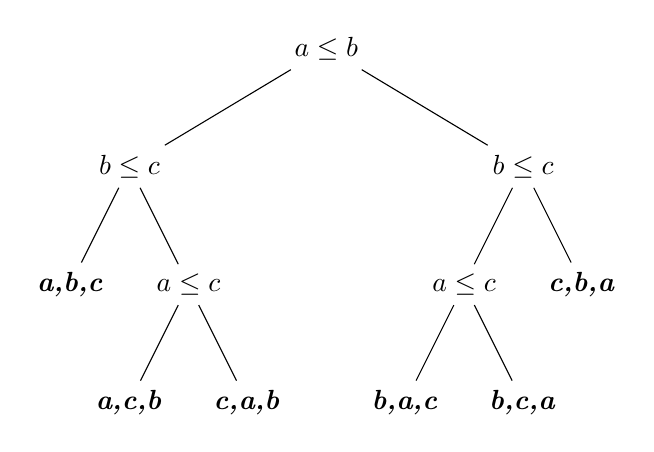
\begin{tikzpicture}[level distance=1.5cm,
  level 1/.style={sibling distance=5cm},
  level 2/.style={sibling distance=1.5cm},
  level 3/.style={sibling distance=1.5cm}]
  \node {$a \leq b$}
    child {node {$b \leq c$}
        child {node {\textbf{\textit{a,b,c}}}}
        child {node {$a \leq c$} {
          child {node {\textbf{\textit{a,c,b}}}}
          child {node {\textbf{\textit{c,a,b}}}}
      }}
    }
    child {node {$b \leq c$}
        child {node {$a \leq c$} {
          child {node {\textbf{\textit{b,a,c}}}}
          child {node {\textbf{\textit{b,c,a}}}}
      }}
          child {node {\textbf{\textit{c,b,a}}}}
    };
\end{tikzpicture}
\end{center}

Observe that the height or depth of the tree represents the amount of computations which must be performed.
Furthermore the height of the tree is not the same for every leaf node (computation result).\\

This is because we can prune some branches due to the transitive property of $\leq$,
given $a \leq b$ and $b \leq c$ we also know that $a \leq c$ is true.
Thus we do not need to compute $a \leq c$.
Conversely given $a \leq b$ and $c \leq b$ we \textbf{do not know}
anything about $a \leq c$.
This is another computation we need to perform to have a correct ordering.\\

Obviously this tree is correct for $n = 3$, so we can say
the complexity lower bound for $n = 3$ is 3 computational steps.
This is because equipped with only comparison we can only go in one
of two directions after each computation (true or false),
and we must be able to produce all six possible orderings.

Well for a three item set $(a,b,c)$ there exists precisely $!3 = 6$ orderings,
or more generally there exists for an $n$ item set $!n$ orderings.
Because this model of computation is binary decision trees,
we can only have $2^x$ leafs (or results) given $x$ computations,
however we need $!n$ leafs therefore, given this information
we can show that comparison sorting has $\Omega(n log_2 n)$.
\begin{align*}
    2^x &\geq !n \\
    x &\geq \log_2(!n) \\
    \log_2(!n) &= \log_2n + \log_2(n − 1) + \dots + \log_2(2)\\
               &= \Omega(n\log_2n)
\end{align*}

\subsection{Algebraic Computation Trees}
\textbf{Algebraic Computation Trees: Examples}\\
We can expand the decision tree model to something more powerful.
Consider the problem of finding if a point is inside the unit circle:
\begin{itemize}
    \item \textbf{Input}:A point $(x,y) \in \mathbb{R}^2$
    \item \textbf{Output}: Yes iff $x^2 + y^2 \leq 1$
\end{itemize}

\begin{center}
    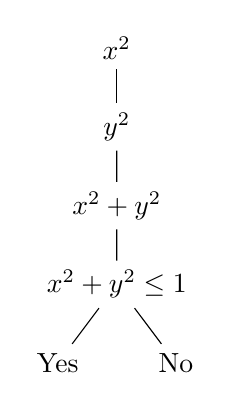
\begin{tikzpicture}[level distance=1cm,
  level 1/.style={sibling distance=2cm},
  level 2/.style={sibling distance=1.5cm},
  level 3/.style={sibling distance=1.5cm},
  level 4/.style={sibling distance=1.5cm},
  level 5/.style={sibling distance=1.5cm}]
  \node {$x^2$}
        child {node {$y^2$}
        child {node {$x^2 + y^2$}
        child {node {$x^2 + y^2 \leq 1$}
            child {node {Yes}}
            child {node {No}}
            }}
        };
\end{tikzpicture}
\end{center}

The complexity of this algorithm (the height of the tree) is 4, i.e., a constant.
This is quite natural since we assume that the size of the input is a constant.
To further generalise our algebraic computation trees,
we will say that every node, except leaves, have three children.
The children correspond to the computation being $(= 0), (< 0), (> 0)$.

\begin{center}
    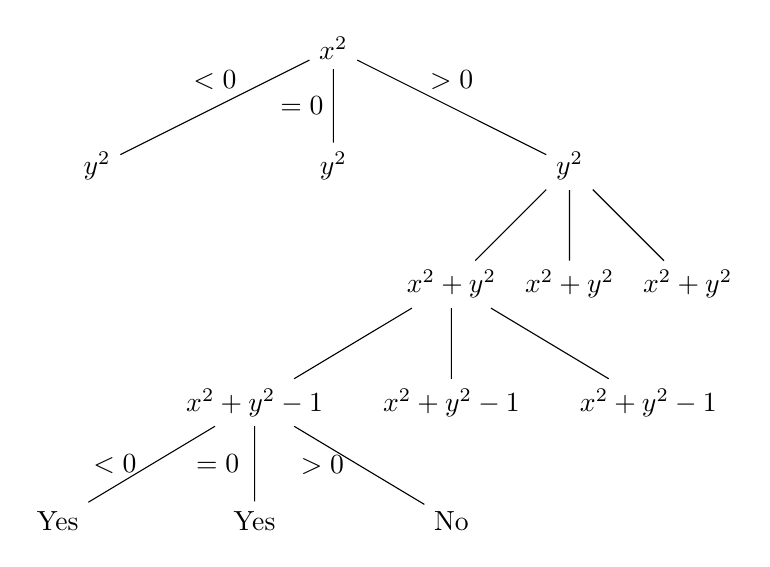
\begin{tikzpicture}[level distance=1.5cm,
  level 1/.style={sibling distance=3cm},
  level 2/.style={sibling distance=1.5cm},
  level 3/.style={sibling distance=2.5cm},
  level 4/.style={sibling distance=2.5cm}]
    \node {$x^2$}
            child {node {$y^2$} edge from parent node[left,above=3pt] {$< 0$}
            }
            child {node {$y^2$} edge from parent node[left] {$= 0$}
            }
            child {node {$y^2$}
                child { node {$x^2 + y^2$} 
                    child { node {$x^2 + y^2 - 1$} 
                        child { node {Yes} edge from parent node[left=2pt] {$< 0$}}
                        child { node {Yes} edge from parent node[left=2pt] {$= 0$}}
                        child { node {No}  edge from parent node[left=2pt] {$> 0$}}
                    }
                    child { node {$x^2 + y^2 - 1$} }
                    child { node {$x^2 + y^2 - 1$} }
                }
                child { node {$x^2 + y^2$} }
                child { node {$x^2 + y^2$} }
            edge from parent node[left,above=3pt] {$> 0$} }
       ;
\end{tikzpicture}
\end{center}

In the example above for the sake of brevity we don't show all the different branches,
simply because we never make any changes to our computation dependent on the result;
that is until the very end where we use it for our yes or no result.
This tree, were it completed, would have $3^4 = 81$ nodes,
much more than our previous tree.
However observe that the height remains unchanged at four,
thus the complexity is the same.\\

One can generalise this example from membership of the unit circle to membership
of the $n$ dimensional unit ball. Simply calculate
$$1 \leq \sum_{i=1}^{n} x_i^2$$
You calculate $x_i^2$ for the $i$-th dimension and add it to the running total;
this takes $2n$ steps.
In case $n = 2$ we get complexity four as our computation tree showed.\\

\textbf{Algebraic Computation Trees: Definition}
\begin{definition}
    A subset $S \subset R^n$ is called \textit{(basic) semi-algebraic} if it is defined by
    $$\{P_1(x_1,\dots x_n) = 0,\dots P_n\}
    \cup
    \{Q_1(x_1,\dots x_n) > 0,\dots Q_m\}$$
    where $P_i$ and $Q_j$ are polynomials in $n$ variables
    i.e., S is a set of all solutions of a system of equations and strict inequalities.
\end{definition}

Algebraic computation tree $T$ in variables $x_1,\dots x_n$
is a tree with the root $v_0$ such that to every vertex $v$ (except leaves)
is an arithmetic operation (addition, subtraction or multiplication) 
and a polynomial $f_v$ is attached.\\

For example $f_3 = f_1 + f_2$ where $f_3$ is the new polynomial;
more precisely in our previous example membership of the unit circle
we have
$$f_1 = x^2 \quad f_2 = y^2 \quad f_3 = x^2 + y^2$$
$$f_4 = f_3 - 1 = x^2 + y^2 - 1$$

\textbf{Semi-Algebraic Sets and Algebraic Computation Trees}\\
Let $v_0, v_1,\dots, v_\omega$ be the sequence of vertices
along the (unique) branch leading from the root $v_0$ to $v_\omega$.
An arithmetic operation at $v_i$ is performed on a pair from
$$\{x_1,\dots x_n\} \cup \{f_0\dots f_{i - 1}\}$$
and the result is at $f_i$.
Note that every $v$ has exactly three children.\\

Let $*_i \in \{>0,=0,<0\}$ for $0 \leq i < \omega$ be the sign of $f_{v_i}$,
One can assign the semi-algebraic set $U_\omega$ to $v_\omega$
$$U_\omega = \{f_0*_00,f_1*_10\dots f_{\omega - 1} *_{\omega - 1}0\}$$

To each leaf $\omega$ of $T$ an output Yes or No is assigned.
We call $U_\omega$ an accepting set if the leaf $\omega$ has the output Yes assigned.
We say that T tests the membership to the union of all accepting sets.\\

To illustrate this relation between
semi-algebraic sets and algebraic computation trees,
consider our unit circle example computations which works as follows.
A specific point $x \in \mathbb{R}^n$ is taken as an input.
Then the value $f_{v_0}(x)$ is computed and the sign of this value is determined.
According to the sign, the algorithm goes to the corresponding child $v_1$ of $v_0$.
If the process eventually arrives to a Yes-vertex, then $x$ belongs to an accepting set,
and, therefore, to the union of all accepting sets.\\

\textbf{Distinctness Problem: Upper Bound}
\begin{itemize}
    \item \textbf{Input}: $(x_0, x_1,\dots x_n) \in \mathbb{R}^n$
    \item \textbf{Output}: Yes iff $\forall\ i,j$ where $0 \leq i,j \leq n, i \neq j$ we have $x_i \neq x_j$
\end{itemize}
An immediate solution for this problem is to sort the numbers $(x_0, x_1,\dots x_n)$
then compare pairwise neighbours for equivalence;
this has complexity $O(nlogn)$.
It is clear that this algorithm can be represented in a form of algebraic computation tree
of the height $O(nlogn)$ (compare with sorting).
We are going to develop a general method for proving lower complexity bounds for algebraic computation trees,
and will apply this method to prove the $\Omega(nlogn)$ lower bound for Distinctness.\\

\textbf{Connected components of Semi-Algebraic Sets}\\
Informally,
a finite union $W$ of semialgebraic sets is called connected
if for every $x, y \in W$ there is a “continuous” curve in $W$ containing both $x$ and $y$.
A formal definition can be found in textbooks on topology.

\begin{definition}
    Any maximal (with respect to the set-theoretical inclusion) connected subset of W is called connected component of W.
\end{definition}

\begin{theorem}
    Every finite union $W$ of semialgebraic sets
    can be uniquely represented as a union of a finite number of its connected components
    (which are finite unions of semialgebraic sets):
    $$W = \bigcup\limits_{1\leq i \leq k} W_i$$
\end{theorem}

\begin{example}
    Consider these examples
    \begin{enumerate}
        \item The union of open intervals $W = (0, 1) \cup (2, 3) \subset R$ is \textbf{not connected}.
            Intervals $(0, 1)$ and $(2, 3)$ are connected components of W .
        \item The union $W = (0, 1) \cup (1, 2)$ is \textbf{not connected} with $(0, 1),\ (1, 2)$ being $W$’s connected components.
        \item The union $W = (0, 1) \cup 1 \cup (1, 2) = (0, 2)$ \textbf{is connected} and is its own unique connected component.
        \item The semialgebraic set $W = \{X \neq Y \} \in R^2$
            (which also can be written in the form $W = \{X^2 − 2XY + Y^2 > 0\}$)
            is \textbf{not connected} and has two connected components: $\{X − Y > 0\}$ and $\{Y − X > 0\}$.
    \end{enumerate}
\end{example}

\begin{theorem}
    Projection of a connected set $W \subset \mathbb{R}^{n+m}$
    on a coordinate subspace $\mathbb{R}^n$ is also connected.
\end{theorem}

\textbf{Lower Bound for Membership to a Semi-Algebraic Set: Decision Computation Trees}

\begin{definition}
    Let the union $\Sigma$ of all accepting sets
    of an algebraic computation tree $T$
    have $\nu(\Sigma)$ connected components.
\end{definition}

\begin{theorem}
    The height $k$ of a \textbf{decision computation tree} $T$,
    i.e. the complexity of testing membership to $\Sigma$,
    is $\Omega(\log\nu(\Sigma))$.
\end{theorem}

\begin{proof}
    Observe that any non-empty accepting set $W$ of $T$
    is a set of all points in $\mathbb{R}^n$ satisfying a system of linear equations and strict linear inequalities,
    and is, therefore, a convex polyhedron in $\mathbb{R}^n$.  It follows that
    $$\nu(W) = 1$$
    Since there is at most $3^k$ leaves in $T$, we get
    \begin{align*}
                3^k &\geq \nu(\Sigma) \\
                  k &\geq c\log \nu(\Sigma)
    \end{align*}
    Taking the binary logarithm in both parts,
    we obtain an inequality for a constant $c > 0$,
    hence we have
    $$\Omega(\log\nu(\Sigma))$$
\end{proof}

\textbf{Thom-Milnor’s bound}
\begin{theorem}
    \textit{(R. Thom, J. Milnor)}
    Let a semialgebraic set $W$ be defined by a system of
    equations and strict inequalities with polynomials of degree at most $d$ in $n$ variables,
    having $m$ inequalities.
    Then the number of all connected components of $W$ does not exceed
    $$((m + 1)d)^{cn}$$
    for a constant $c > 0$.
    The known proofs of Thom-Milnor’s bound use complex arguments from differential and algebraic topology,
    we are not considering them.
\end{theorem}

\begin{theorem}
    Let $W$ be a semialgebraic set satisfying the conditions of the theorem.
    Then the number of the connected components of a projection of $W$ on any coordinate subspace does not exceed
    $$((m + 1)d)^{cn}$$
    for a constant $c > 0$.
\end{theorem}

\begin{theorem}
    \textit{(M. Ben-Or)}
    Let the union $\Sigma$ of all accepting sets of an \textbf{algebraic computation tree} $T$
    have $\nu(\Sigma)$ connected components.
    Then the height $k$ of $T$ (the complexity of testing membership to $\Sigma$) is
    $$\Omega(\log(\nu(\Sigma)) − n)$$
\end{theorem}

\textbf{Distinctness problem: lower bound}
\begin{theorem}
    Distinctness problem has a complexity lower bound $\Omega(n \log n)$.
\end{theorem}
\begin{proof}
    The union $\Sigma$ of all accepting sets in this problem
    is the complement to the union of hyperplanes defined by
    all possible linear equations of the kind
    $$X_i = X_j$$
    where $i \neq j$,
    in other words,
    at a point $x = (x_1, \dots x_n) \in \Sigma$ all coordinates are pairwise distinct
    (briefly consider the to $W = \{X \neq Y \} \in R^2$).
    Herewith, the coordinates of $x$ are somehow ordered:
    $$x_{i_1} < \dots < x_{i_n}$$
    It is easy to see that,
    at each point of a connected component $\Sigma_i$ of $\Sigma$
    the order of the coordinates is the same.
    Indeed, suppose this is wrong, and for two points
    $$y = (y_1, \dots , y_n)\quad z = (z_1, \dots , z_n)$$
    we have $y_l < y_m$,
    but $z_l > z_m$.
    By the definition of connectedness,
    there is a continuous curve in $\Sigma_i$ connecting $y$ and $z$.
    Since the values of coordinates change continuously along the curve,
    there should be a point $w = (w_1, \dots , w_n)$ on the curve such that $w_l = w_m$.
    Thus, $w \in {X_l = X_m}$,
    that is, $w$ belongs to the complement of $\Sigma$, which is a contradiction.\\

    We have proved that the number of connected components of $\Sigma$
    is not less than the number $n!$ of all permutations of $n$ coordinates (in fact these numbers coincide).
    According to the Thom-Milnor’s theorem, we get a lower bound
    \begin{align*}
        &\Omega(\log(n!)) \\
        &\Omega(n \log n)
    \end{align*}
\end{proof}


\pagebreak
\section{Quantum Complexity}
\textbf{Complex Numbers}\\
Complex numbers play a very special role in quantum computing.
A complex number may have three principal representations.\\

\textbf{Pair Representation}\\
As a pair of real numbers $(a, b)$, traditionally written as $a + ib$,
where $a, b \in R$ and $i$ is \textit{a posteriori} interpreted as $\sqrt{-1}$.
Arithmetic operations of $+$ and $\times$ are defined as
\begin{align*}
    (a+ib) +      (c+id) &= (a+c)   + i(b+d)  \\
    (a+ib) \times (c+id) &= (ac−bd) + i(ad+bc)
\end{align*}
Observe this is consistent with our definition $i=\sqrt{-1}$.
$$i^2 = (0 + i)(0 + i) = −1$$

\textbf{Polar Representation}\\
A complex number $z = a + ib$ has a natural representation
as a vector $(a,b)$ in the real plane $R^2$.
The norm of this vector, $|z| = \sqrt{a^2 +b^2}$,
is called the \textit{modulus} or \textit{magnitude} of $z$,
while the angle $\varphi = arctan(b/a)$ between vector $(a, b)$
and the positive direction of the horizontal axis is called the argument of $z$.
The pair $(m,\varphi)$ completely determines z and is called polar representation of z.
Note that in physics literature modulus is usually called magnitude, while argument is called phase.
We pass from polar representation (m, $\varphi$) to the original representation a + ib via formulas:
a = m cos $\varphi$, b = m sin $\varphi$.
A formula for multiplication of two complex numbers is particularly
easy in the polar representation:
$$(m_1, \varphi_1) \times (m_2, \varphi_2) = (m_1 \times m_2, \varphi_1 + \varphi_2)$$

\textbf{Exponential Representation}\\
From $a = m cos \varphi$, $b = m sin \varphi$ we deduce that
$$a + ib = m(cos\varphi + isin\varphi)$$
According to the Euler formula,
$$cos\varphi + isin\varphi = e^{i\varphi}$$
where $e = 2.71828\dots$
This leads us to the exponential representation:
$a + ib = me^{i\varphi}$
Multiplication formula in this case is
$$m_1e^{i\varphi_1} \times m_2e^{i\varphi_2} = m_1m_2e^{i(\varphi_1+\varphi_2)}$$
For a complex number $z = a + ib$ its complex conjugate is the number $\bar{z} = a − ib$.
It is clear that if $z \in R$, then $\bar{z} = z$, i.e. $b = 0$.

\textbf{Vectors and matrices}\\
We consider an $n$-dimensional vector space $C^n$ over complex numbers.
Its elements are column vectors $z = (z_1,\dots,z_n)^T$,
where every $z_i \in C$.

In physics (and quantum computing) vector $z$ is also denoted by \textit{ket-notation},
$|z\rangle$.
There is also a sister \textit{bra-notation}, $\langle z|$,
standing for the row vector $(\bar{z_1}, \dots , \bar{z_n})$.
The \textit{bra-ket (bracket) notation} was introduced by P. Dirac.

The notation $\langle x|y \rangle$,
for two vectors $x = (x1, . . . xn)$ and $y = (y1, . . . yn)$,
means the dot (inner) product of these vectors,
namely the number x1y1 + · · · + xnyn.
The notation $|y\rangle\langle x|$ also has some meaning.
%There is also a sister bra-notation, ⟨z|, standing for the row vector (z ̄1, . . . , z ̄n). The bra-ket (bracket) notation was introduced by P. Dirac. The notation ⟨x|y⟩, for two vectors x = (x1, . . . xn) and y = (y1, . . . yn), means the dot (inner) product of these vectors, namely the number x ̄1y1 + · · · + x ̄nyn. The notation |y⟩⟨x| also has some meaning, discussed later.
As usual, linear maps between vector spaces are described by matrices,
in our case having complex numbers as elements.
We will need the following special types of matrices.
\begin{itemize}
    \item Given a matrix A,
    its adjoint matrix,
    A†, is defined as (A)T = AT ,
    where the bar denotes element-wise complex conjugation.
    \item A matrix A is Hermitian if A† = A. Observe that A is a square matrix, and all its diagonal elements are real numbers.
    \item A square matrix U is unitary if UU† = U†U = I,
    where I is the identity matrix of the appropriate size. In other words, a matrix is unitary if its adjoint is inverse.
\end{itemize}

$$
\begin{pmatrix}
    cos\ \alpha & -sin\ \alpha  \\
    sin\ \alpha & cos\ \alpha
\end{pmatrix}
$$
$$
\frac{1}{\sqrt{2}}
\begin{pmatrix}
    1 & 1  \\
    1 & -1
\end{pmatrix}
$$
\textbf{Qubits}\\
\textbf{Bloch sphere}\\
\textbf{Multiple Qubits}\\
\textbf{Functions from bits to bits}\\
\textbf{Deutsch’s Algorithm}\\


\end{document}
